\documentclass{article}
\pagestyle{headings}

\usepackage[portuguese]{babel}
\usepackage[utf8]{inputenc}
\usepackage[T1]{fontenc}

\usepackage{graphicx}

\title{A teoria do perigo aplicada à detecção de fraude}
\author{Bruno Barcarol Guimarães}

\begin{document}

\maketitle
\newpage

\tableofcontents{}
\newpage

\section{Introdução}

\paragraph{}O crescente avanço na tecnologia de armazenamento de dados, principalmente em termos de velocidade e tamanho, permite a criação de bancos de dados complexos e detalhados. Com isso, o desenvolvimento de programas de computador que há anos atrás seriam computacionalmente inviáveis torna-se possível. Uma área fortemente influenciada por esse fator é a mineração de dados. Definida como ``análise de bases (geralmente extensas) de dados previamente coletados para estabelecer relações e apresentar a informação de forma mais clara e útil ao proprietário dos dados''\footnote{``Data mining is the analysis of (often large) observational data sets to find unsuspected relationships and to summarize the data in novel ways that are both understandable and useful to the data owner.''. HAND, D. J.; MANILLA, H.; SMYTH, P. 2001. \emph{Principles of data mining}. p. 1.}, a mineração de dados é associada à ideia do aproveitamento de grandes bases de dados para auxiliar o profissional em alguma tarefa, através da apresentação de padrões e relações que seriam difíceis ou impossíveis de serem encontrados pelo observador humano.

\paragraph{}Os exemplos da sua utilização são inúmeros, estendendo-se virtualmente a qualquer atividade, de empresas comerciais à medicina e engenharia. Cada vez mais informação coletada e armazenada, e a análise torna-se impossível sem o uso de uma ferramenta automatizada para sintetizá-la. A mineração extrai padrões ou modelos dessas fontes de informação, apresentando informação que pode ser utilizada gerando alguma vantagem para o detentor dos dados. Isso tem motivado pesquisadores a desenvolver algoritmos capazes de identificar esses padrões com mais detalhamento e significado.

\paragraph{}Como área interdisciplinar, a mineração atrai estudiosos de diversas áreas da computação como, em especial, a Inteligência Artificial (IA). A combinação de técnicas tradicionais de mineração com os algoritmos desta área estende em muito o seu poder de análise e sintetização. Até a definição mais básica da Inteligência Artificial já mostra que as duas áreas têm objetivos em comum, como a ``tentativa de definição'' de Luger:

\begin{quote}
``Inteligência Artificial (IA) pode ser definida como a área da ciência da computação que se dedica a automação de comportamento inteligente.''\footnote{``Artificial intelligence (AI) may be defined as the branch of computer science that is concerned with the automation of inteligent behaviour.''. LUGER, G. F. 2008. \emph{Artificial Intelligence: Structures and Strategies for Complex Problem Solving}. p. 1.}
\end{quote}

\paragraph{}Analisar informações, raciocinar e tirar conclusões são também objeto de estudo da Inteligência Artificial, e muitos dos seus métodos podem ser usados em conjunto com a mineração. De fato, as grandes bases de dados que geralmente são objeto de atuação da mineração constituem excelente campo de testes para os algoritmos da IA. Redes neurais e bayesianas, clustering e lógica nebulosa (fuzzy) são alguns dos métodos mais aplicados nessas situações.

\paragraph{}Com frequência, nas ciências, pesquisadores se voltam a áreas diferentes das suas próprias, com o objetivo de encontrar soluções para os seus problemas adaptando outras soluções. Um exemplo disso, na Inteligência Artificial, são os Sistemas Imunológicos Artificiais, inspirados no sistema imunológico natural. Conforme definiu Castro:

\begin{quote}
``\emph{Sistemas Imunológicos Artificiais (SIA) são sistemas adaptativos, inspirados na teoria da imunidade e funções, princípios e modelos imunológicos observadas, que são aplicados à resolução de problemas.''\footnote{``Artificial Immune Systems (AIS) are adaptive systems, inspired by theoretical immunology and observed immune functions, principles and models, which are applied to problem solving.''. CASTRO, L. N.; TIMMIS, J. 2002. \emph{Artificial Immune Systems: A New Computational Intelligence Approach.} p. 57.}}
\end{quote}

\paragraph{}A utilização desse tipo de sistema é nova, até dentro da área de Inteligência Artificial: os primeiros trabalhos nessa área foram desenvolvidos a partir da metade dos anos 90. Mesmo assim, é uma técnica que apresenta bons resultados e tem despertado o interesse de pesquisadores. Uma adição ainda mais recente foi a da Teoria do Perigo, proposta por Matzinger, em 1994. A principal revolução na Teoria do Perigo é a mudança na forma como as células tomam conhecimento e reagem, introduzindo a noção de perigo e tolerância.

\paragraph{}Uma área que têm recebido crescente atenção de estudos de mineração de dados e Inteligência Artificial é a de segurança. O reconhecimento de padrões e capacidade de investigação de grandes bases de dados são os maiores desafios que profissionais da segurança enfrentam, não apenas na área da informática, mas de forma geral. O desenvolvimento de ferramentas de mineração é visto como um forte candidato à solução desses problemas. O ganho que um profissional tem ao utilizar uma ferramenta dessa natureza é enorme: a tarefa de análise de bases de dados extensas é passada dele para o computador. Nesse sentido, o objetivo é relevar à maquina cada vez mais o trabalho mecânico, para que o ser humano possa se dedicar à análise crítica do material compilado.

\paragraph{}Dentro da segurança, escolheu-se uma área mais específica para delimitar o escopo do trabalho. A detecção de fraude consiste na identificação de padrões e comportamentos associados à atividades irregulares, prevenindo que elas se concretizem. A aplicação de técnicas de mineração de dados em aplicações desse tipo proporcionou espaço para o desenvolvimento de incontáveis trabalhos4. No entanto, a utilização de Sistemas Imunológicos Artificiais ainda é pouco explorada. Viu-se nesse fato uma oportunidade de exploração nesse trabalho.

\subsection{Objetivos}
\subsection{Organização}
\newpage

\section{Fundamentação teórica}

\subsection{Sistemas imunológicos e a teoria do perigo}

\paragraph{}O primeiro modelo do sistema imunológico foi o da distinção entre o próprio e o não-próprio, proposto por Burnet\footnote{BURNET, F. M. 1959. \emph{The Clonal Selection Theory of Acquired Immunity}.}. Ao longo do tempo, novos modelos foram criados, tentando resolver as questões que os outros modelos não explicavam, destancando-se o modelo do não-próprio infeccioso, de Janeway\footnote{JANEWAY, C. A. 1989. \emph{Approaching the Asymptote? Evolution and Revolution in Immunology}.}.

\paragraph{}Uma adição ainda mais recente foi a da Teoria do Perigo. Matzinger\footnote{MATZINGER, P. 1994. \emph{Tolerance, Danger and the Extended Family.}} defende a teoria de que não é a separação do próprio e do não-próprio a força que impulsiona o sistema imunológico, mas sim o que ela caracteriza como ``perigo'': qualquer coisa que cause estresse ou morte não-apoptética (não natural) da célula. Embora não seja completa, essa teoria explica fenômenos que outras teorias sobre o sistema imunológico não explicavam, como o fato de não haver reação contra bactérias no intestino ou na comida, a mudança do conceito de próprio durante a vida e a problemática da própria definição do próprio e do não-próprio.

\paragraph{}Mais do que isso, a teoria do perigo muda a forma como se enxerga o sistema imunológico como um todo: um sistema responsável por manter o corpo em estado de equilíbrio. Dessa forma, a distinção explícita do próprio se torna desnecessária. Discriminação ainda existe, mas seu foco é o perigo, não mais o estranho. O modelo ainda provê explicações para outros fenômenos, como a tolerância a organismos externos mas inofensivos e a eliminação de células próprias.

\paragraph{}O funcionamento do sistema imunológico, conforme a teoria do perigo, é apresentado na figura abaixo\footnote{MATZINGER, P. \emph{op. cit.}}. Os linfócitos B são os responsáveis pela identificação de antígenos através de receptores em sua superfície. Durante uma infecção, essas células se multiplicam e produzem anticorpos para eliminar os antígenos identificados. Elas são capazes de adaptar-se a virtualmente qualquer tipo de antígeno. Um outro tipo de linfócito, os linfócitos T, quando ativados, podem exercer uma de duas funções: os linfócitos T citotóxicos (CTL) são responsáveis pela eliminação de células infectadas, enquanto que os linfócitos T auxiliares (Th) são responsáveis pela ativação de outras células, entre elas os linfócitos B. Além disso, alguns linfócitos T são mantidos como células de memória. Existe ainda um outro tipo de linfócito, o T \emph{killer} (Tk), que não tem receptores antígeno-específicos, mas é capaz de reconhecer células infectadas e algumas células anormais. O objetivo dessas células é atuar como a primeira defesa contra infecções, e são muito importantes nos começo da vida.


\begin{figure}[h]
\centering
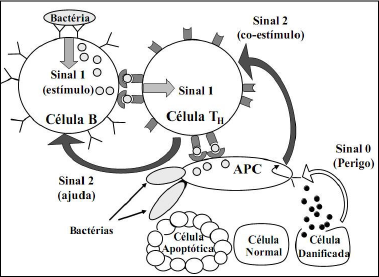
\includegraphics[scale=0.75]{img/danger_theory.png}
\caption{O sistema imunológico}
\end{figure}

\paragraph{}O comportamento dos linfócitos T e B se baseia em três regras:

\begin{enumerate}
\item Linfócitos T e B entram em atividade ao receber os sinais um e dois, morrem ao receber apenas o sinal um e ignoram o sinal dois sem o recebimento do sinal um.
\item Linfócitos T aceitam o sinal dois apenas de APCs, enquanto os linfócitos B, apenas de linfócitos T ativos ou células de memória. O sinal um pode ter origem em qualquer célula.
\item Linfócitos T ativados não precisam do sinal dois para entrarem em ação. Após um período de tempo, elas voltam ao estado de repouso, necessitando novamente dos dois sinais.
\end{enumerate}

\paragraph{}Células Apresentadoras de Anítgeno (ATP, ou Antigen Presenting Cell) são as células responsáveis por apresentar os antígenos às células T. Essas células podem ser os linfócitos B, macrófagos e as células dendríticas. Quando as células se encontram em estado de estresse ou morrem de forma não programada, enviam um sinal para as células APC, representado pela seta Sinal 0. Isso desencadeia o envio do sinal dois para os linfócitos Th. Enquanto isso, linfócitos B usam seus receptores para reconhecer antígenos nas suas redondezas, enviando o sinal um para os linfócitos Th. É o par de sinais um (reconhecimento do antígeno) e dois (sinal enviado pelo linfócito T, ativado pelo sinal de perigo) que faz com que a reação imunológica tenha início.

\subsection{Problema: detecção de fraude}
\section{Proposta}
\subsection{Objetivos}
\subsection{Arquitetura}
\subsection{Critérios}
\subsection{Resultados}
\section{Conclusão}
\subsection{Síntese}
\subsection{TCC II}

\end{document}

